\documentclass[main.tex]{subfiles}

\begin{document}
    \chapter{Introduction}
    \setlength{\epigraphwidth}{0.8\textwidth}
    % \epigraph{
    %         \selectlanguage{greek}
    %         >en p~asi g`ar to~is fusiko~is >'enest'i ti jaumast'on\\
    %         \vspace{0.2cm}
    %         \selectlanguage{english}
    %         In all things of nature there is something of the marvelous
    % }{--- Aristotle, 384-322 BC}
        \epigraph{
            \selectlanguage{english}
            ``You must have chaos within you to give birth to a dancing star''
    }{--- Friedrich Nietzsche, Thus Spoke Zarathustra}
    % \vspace{2cm}


    From the early days when astronomers gazed at the night sky to the present era of cutting-edge instruments and sophisticated computational models, our comprehension of the structure and evolution of stars has grown exponentially. Although many fundamental processes are still poorly understood (e.g., the theory of convection and internal mixing, the effects of rotation and magnetic fields), improvements in both the quantity and quality of observational data, coupled with significant progress in theoretical advancements and the adoption of novel computational techniques, have allowed for an enormous expansion and refinement of both the formal and conceptual basis of the subject.

    In this introductory chapter, we investigate the fundamentals of stellar astrophysics, examining how stars evolve from their formation to their eventual transformation into compact stellar remnants. During this exploration, we focus particularly on neutron stars, which hold significant importance in astrophysics. Formed from the remnants of dying stars, neutron stars serve as unique celestial laboratories, providing valuable insights into the nature of matter and the effects of strong gravity. This dissertation aims to contribute to our understanding of neutron stars by investigating the intricate processes that govern their life cycles, with a specific emphasis on their structure and mass distribution.

    Naturally, it has been necessary to be selective in the material presented. The intention here is to lay the groundwork and provide a succinct overview of key concepts tailored to the dissertation's scope, steering away from an exhaustive exploration of stellar astrophysics principles. However, readers seeking further clarification may find additional resources in classical textbooks that offer extensive coverage across diverse facets of this field \citep[e.g.,][]{Clayton, Prialnik, Eggleton, Kippenhahn, Carroll_Ostlie_2017}.

    
    {\hypersetup{linkcolor=black, pdfborder=0 0 1}
    \adjustmtc
    \adjustmtc
    \minitoc
    \newpage
    }
    
    
    
    \section{A Brief Introduction to Stellar Structure \& Evolution}\label{sec:ch1:intro}
    From humanity's standpoint, stars often appear as timeless entities, seemingly having existed for eternity and destined to persist indefinitely in the vast expanse of the Universe. This perception, however, is an illusion, stemming from the limited time span during which we observe these celestial bodies in relation to their overall lifetime. In reality, stars undergo the complex processes of birth, evolution, and eventual demise within the cosmic landscape, unfolding over timescales beyond human intuition. To comprehend the evolution of stars over time, observational studies inherently rely on short-term measurements taken from extensive populations.
    Consider the analogy of a paleoanthropologist studying the biological and cultural evolution of humans throughout history. With the first appearance of Homo sapiens believed to have occurred approximately \SI{200000}{years} ago, the only viable method for such a study is through the examination of a large population of fossil records and archaeological evidence spanning different evolutionary stages.

    Given a large sample of stars, we may construct the so-called \textit{``Hertzsprung-Russell diagram''} (H-R diagram), where stars' luminosity is plotted against their effective surface temperature\footnote{It is worth noting that variations of the H-R diagram exist. In alternative forms, the diagram may employ color, magnitude, or spectral type on its axes. For instance, a Color-Magnitude Diagram (CMD) is a variation that plots stars based on their color and magnitude, providing insights into stellar populations and evolutionary stages based on these observable characteristics.}, an example of which can be seen in Fig.~\ref{fig:hrd_gaia}. This diagram provides a visual representation of stellar characteristics, allowing us to organize and analyze large populations of stars simultaneously. Through the H-R diagram, stars can be classified based on their luminosity, temperature, and evolutionary stage, providing a comprehensive snapshot of various stellar life cycles. Much like the paleoanthropologist's careful examination of diverse fossil records, the H-R diagram offers astronomers a panoramic view of stellar evolution, enabling them to unravel the mysteries embedded in stellar dynamics.

    \begin{figure}[h!]
        \centering
        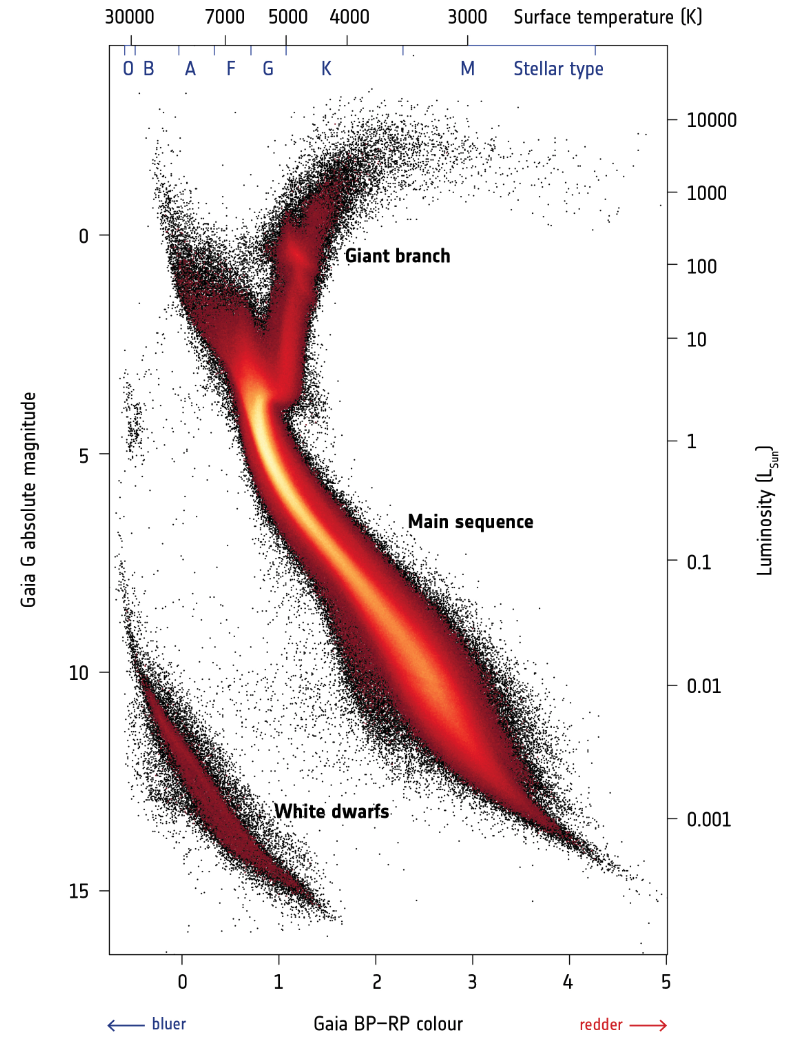
\includegraphics[scale=0.25]{figures/chapter1/hrd_gaia.png}
        \caption{Hertzsprung-Russell diagram obtained by a selection of stars from the second release catalogue of ESA's Gaia satellite. Copyright: \href{https://sci.esa.int/web/gaia/-/60198-gaia-hertzsprung-russell-diagram}{ESA/Gaia/DPAC}}
        \label{fig:hrd_gaia}
    \end{figure}

    Upon a casual observation of Fig.~\ref{fig:hrd_gaia}, it becomes evident that stars are not randomly distributed on the H-R diagram but instead cluster, forming distinct structures primarily based on their masses, chemical composition, and evolutionary stage. The most prominent of these structures is a large collection of stars forming a diagonal stripe known as the \textit{``main sequence''}. Above the main sequence lies another feature referred to as the \textit{``giant branch''}, while below the main sequence, stars are distributed on the left-hand side, forming a group of objects known as \textit{``white dwarfs''}. The presence of these structures on the H-R diagram implies the existence of underlying physical laws governing these observational characteristics, which will hopefully become apparent in the following sections.

    

    \newpage
    \subsection{Stars in Isolation: From Birth to Death}
    This section provides a broad overview of the life cycle of individual stars, encompassing their birth through their eventual demise. While we will touch upon the processes occurring within the stellar interior, such as energy generation mechanisms, the significant impact of other factors, such as mixing and rotation, on stellar evolution will be explored in more detail in a subsequent section.
    
    \subsubsection{Star formation}
    The life of a star is the story of a cosmic tug-of-war between gravity and the star's internal pressure. This story begins within giant molecular clouds, an agglomeration of interstellar gas and dust. These molecular clouds are often composed of hydrogen molecules, helium, and trace amounts of other elements\footnote{In astronomy, elements heavier than helium are commonly grouped under the term ``metals'', although this classification doesn't necessarily reflect their chemical properties. The abundance of these heavier elements within celestial structures, such as stars, is quantified by the term ``metallicity''.}, serving as the cosmic nurseries where stars are born (see Fig.~\ref{fig:rho_ophiouchi}).
    Initially, the molecular cloud is in a state of equilibrium, where thermal motions, driven by temperature, work to resist the force of gravity that seeks to collapse the cloud. The interplay between these opposing forces is described by the \textit{virial theorem} which, under the assumption that the cloud behaves as an ideal gas, takes the form:
    \begin{equation}\label{eq:virial}
        2T + U = 0,
    \end{equation}
    where $T$ is the kinetic energy and $U$ is the gravitational potential of the system. For as long as this equation holds true, the system will neither expand nor collapse. If the kinetic energy term dominates, then the thermal pressure overcomes the gravitational attraction and the system will expand. On the other hand, if the gravitational potential term dominates, the system will contract on the free-fall (dynamic) timescale:
    \begin{equation}\label{eq:dynamical_timescale}
        \tau_\mathrm{ff} \propto (G\bar{\rho})^{-1/2},
    \end{equation}
    i.e., the characteristic time that would take a body to collapse under its own gravity. Here $G$ is the gravitational constant and $\bar{\rho}$ is the average density of the cloud. Owing to the extremely low densities that characterize molecular clouds, the free-fall timescale is of the order of million of years.

    \begin{figure}[t]
        \centering
        \includegraphics[scale=0.08]{figures/chapter1/Rho_Ophiuchi_cloud_complex.jpg}
        \caption{The $\rho$-Ophiouchi cloud complex, one of the closest star-forming regions to our Solar System, located at the constellation of Ophiuchus. The photograph is a compilation of distinct exposures gathered by the James Webb Space Telescope through the utilization of the NIRCam instrument. Copyright: \href{https://www.esa.int/ESA_Multimedia/Images/2023/07/Rho_Ophiuchi_cloud_complex}{NASA, ESA, CSA}}
        \label{fig:rho_ophiouchi}
    \end{figure}

    By applying the virial theorem, it can be shown that there exists a critical mass threshold, known as the ``Jeans mass'' ($M_J$), which characterizes the point at which self-gravity becomes dominant, overcoming thermal pressure. The Jeans mass is expressed by the formula:
    \begin{equation}\label{eq:jeans_mass}
        M_J \approx \left(\frac{3}{4\pi \rho}\right)^{1/2} \left(\frac{5kT}{G\mu m_H }\right)^{3/2}, 
    \end{equation}
    where $k$ is the Boltzmann constant, $T$ is the temperature of the molecular cloud, $G$ is the gravitational constant, $\rho$ is the density of the cloud, $\mu$ is the mean molecular weight, and $m_H$ denotes the mass of the hydrogen atom.

    Star formation begins as portions of the molecular cloud undergo gravitational collapse, triggered by small irregularities in the distribution of matter. Such density inhomogeneities may be induced by turbulence or external factors, like shockwaves from nearby supernovae and spiral density waves, ultimately leading to gravitational instabilities. Consequently, the molecular cloud fragments into denser regions, surpassing the Jeans mass. These more condensed areas, known as cloud cores, become the sites where individual stars are born and take shape.

    As a molecular cloud core contracts under the influence of gravity, it undergoes an initial phase of isothermal collapse. This phase results in the formation of a \textit{protostellar disk} and, subsequently, a \textit{protostar} at its center. Material continues to accrete onto the protostar, while the surrounding protostellar envelope gradually dissipates over time. This phase plays a critical role in determining the initial mass and angular momentum of the nascent star.
    Throughout this collapse, the core's temperature remains relatively constant due to efficient cooling mechanisms. However, as the density increases, the opacity of the material undergoes a change. In the early stages, when the core is less dense, it is optically thin, allowing radiation to easily escape. However, as the density rises, the core becomes optically thick, hindering radiation from propagating through the increasingly dense material. This shift in opacity significantly influences the thermal balance within the collapsing core\footnote{During this process, energy is generated via the Kelvin-Helmholtz mechanism. The gravitational potential energy liberated due to contraction is radiated away in the form of light.}.
    
    As the core progresses through its evolution, opacity continues to impact its thermal properties. At higher densities, the core transitions from an isothermal collapse to an adiabatic collapse (where cooling can be ignored), leading to a more substantial rise in temperature due to increased opacity. This gives rise to the birth of a protostar within the dense core. The protostar subsequently undergoes further evolution along the Hayashi track\footnote{A trajectory on the Hertzsprung-Russell diagram showcasing the thermal evolution of the protostar during contraction until hydrostatic equilibrium is achieved via central nuclear fusion.}, contracting and heating until the conditions are suitable for the ignition of hydrogen in its center ($T_c \sim 10^7\,\text{}K$). The onset of sustained nuclear fusion in the protostar's core results in the establishment of hydrostatic equilibrium and prevents further collapse. A new star has just been born and has joined the main sequence as a ``\textit{zero age main sequence}'' (ZAMS) star!
    

    \subsubsection{Evolution during the main sequence}
    During the main sequence phase, all stars exhibit a fundamental set of characteristics that define this stable stage in their evolution. Central to this phase is the process of hydrogen burning in the star's core, which involves fusing hydrogen nuclei together to form helium. This nuclear fusion generates a continuous release of energy, establishing a delicate equilibrium between the gravitational forces 
    and the outward pressure gradient generated by the ongoing fusion reactions.

    Two primary mechanisms govern central hydrogen burning in stars: the proton-proton (pp)-chain and the carbon-nitrogen-oxygen (CNO) cycle. In the pp-chain, predominant in lower-mass stars like the Sun, hydrogen nuclei (protons) undergo a series of fusion reactions, ultimately resulting in the conversion of four protons into one helium nucleus, liberating energy in the process. Although the net reaction can be written as:
    \begin{equation}
        \label{eq:pp-chain}
        \mathrm{4\,^1H \longrightarrow \,^4He + 2\,e^+ + 2\,\nu_e + Q(\sim 26.7\,MeV)},
    \end{equation}
    it should be noted that this chain of reactions involves various intermediary steps, including the formation of deuterium and helium-3 as can be seen in Fig.~\ref{fig:pp_cno}.

    \begin{figure}[th!]
        \centering
        \begin{subfigure}{.5\textwidth}
        \centering
        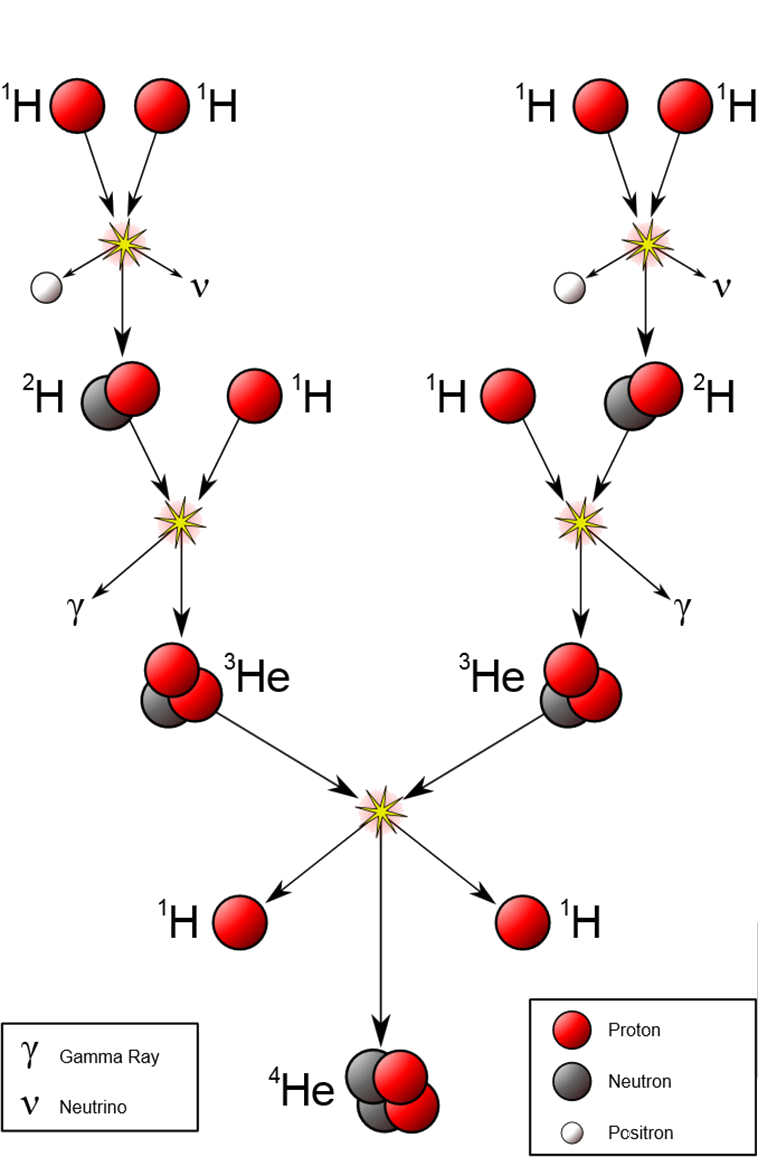
\includegraphics[scale=0.25]{figures/chapter1/pp-chain.png}
    \end{subfigure}%
    \begin{subfigure}{.5\textwidth}
        \centering
        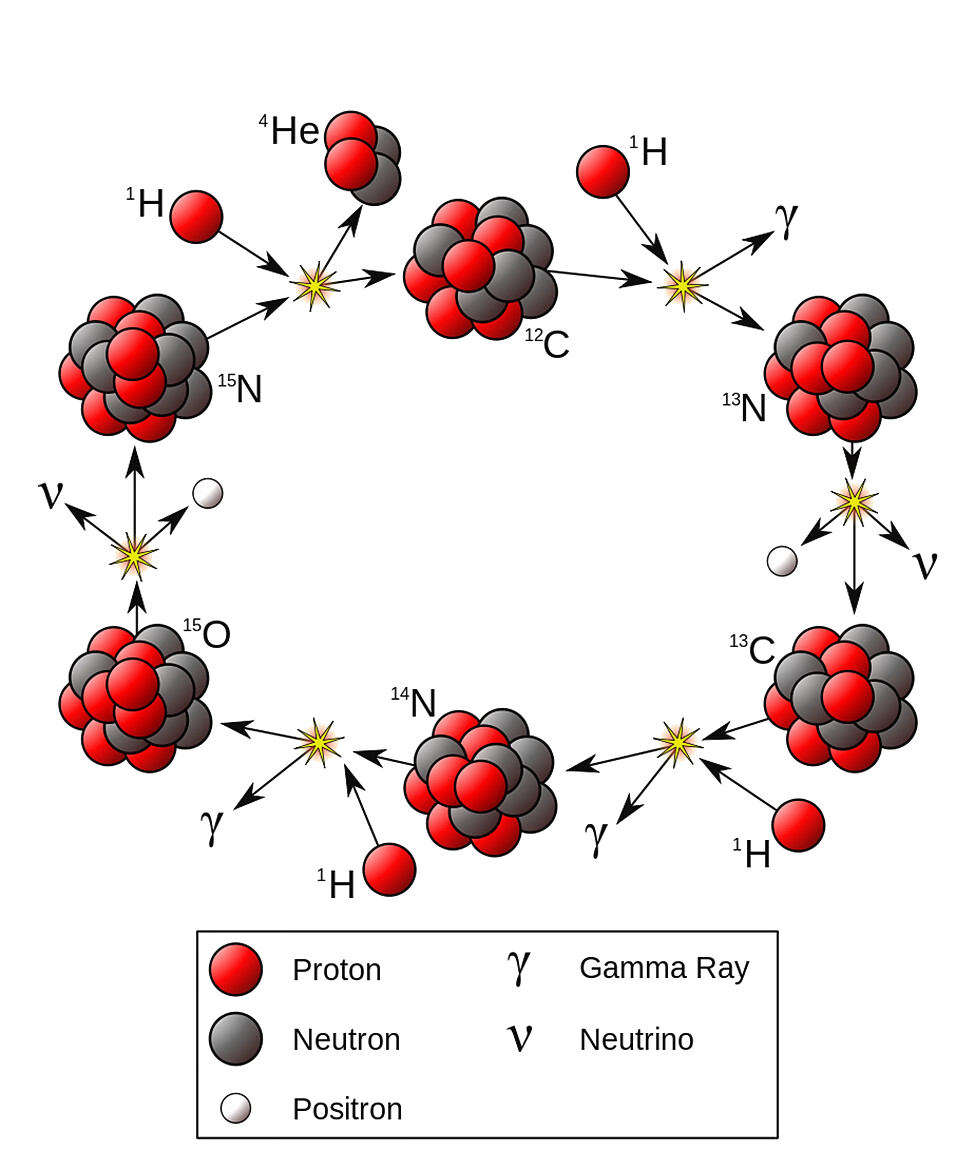
\includegraphics[scale=0.2]{figures/chapter1/cno-cycle.png}
    \end{subfigure}
        \caption{Schematic illustration depicting the primary mechanisms driving energy generation in main sequence stars. On the left, the proton-proton chain is portrayed, while on the right, the CNO cycle is presented. Credit: \href{https://supernova.eso.org/}{ESO Supernova}.}
        \label{fig:pp_cno}
    \end{figure}
    
    Conversely, in higher-mass stars, the CNO cycle becomes a dominant contributor to central hydrogen burning. This cycle involves catalytic fusion reactions facilitated by carbon, nitrogen, and oxygen isotopes acting as catalysts\footnote{The net result of the CNO cycle is the same, regardless of which of these elements initiates the process.}. The CNO cycle is more temperature-sensitive than the pp-chain and becomes increasingly significant in hotter and denser stellar cores. It offers an alternative pathway for hydrogen fusion, enhancing the efficiency of energy production in more massive stars.

    Nevertheless, regardless of the energy generation mechanism, whether it be the pp-chain or the CNO cycle, the temperature and density within the star remain nearly constant until the depletion of hydrogen. The duration of hydrogen burning is determined by the star's mass and luminosity:
    \begin{equation}
        \label{eq:nuclear_timescale}
        \tau_\mathrm{nuc} = \phi f \frac{Mc^2}{L},
    \end{equation}
    known as the ``\textit{nuclear timescale}'', where $M$ is the total mass of the star, $L$ is it's surface luminosity, $c$ is the speed of light, $f$ is the fraction of the total mass of the star that participates in nuclear burning, and $\phi$ is the fractional mass difference of the reaction, i.e., the fraction of the mass that is being converted into energy in each reaction (for hydrogen burning, $\phi \simeq 0.7\%$). Massive stars are vastly more luminous than lower-mass stars; hence, the nuclear timescale on which they burn their hydrogen supplies is of the order of a few million years. On the other hand, the lowest-mass stars may remain in the main sequence for a period that may exceed the current age of the universe. In both cases, however, stars spend most of their lives in this stable phase, which explains the prominence of the main sequence feature on the H-R diagram.
    


    \subsubsection{Evolution after the main sequence}
    After the eventual exhaustion of their energy source, stars that exit the main sequence feature an inert core composed mainly of helium engulfed in a hydrogen-rich mantle. Without the nuclear reactions to provide an outward pressure to counterbalance gravity, the stars' core falls out of equilibrium and begins to contract. As the temperature increases, the conditions become favorable for the ignition of hydrogen in the outer layers surrounding the inert helium core. This external shell burning generates enough energy to cause the layers above it to expand; the radius of the star grows dramatically and it's surface effective temperature decreases, i.e., it appears redder. The star has transformed into a red giant and starts ascending the red giant branch on the H-R diagram.

    In spite that shell hydrogen burning has restored hydrostatic equilibrium by providing support to the outer layers of the star, the inert helium core continues to contract and heat up.
    This transitional stage represents a crucial point in stellar evolution, giving rise to distinct pathways for stars with different masses. In lower-mass stars, the core contracts until electron degeneracy pressure becomes the primary force preventing further collapse instead of thermal pressure. This pressure arises from the Pauli exclusion principle, which prohibits two fermions, such as electrons, from simultaneously occupying the same quantum state. The hydrogen-burning layer above the inert core produces more helium via one of the processes we described earlier. In turn, this helium is accumulated on top of the helium core, allowing it to grow in mass. If the core reaches a critical mass of approximately $0.4\,\msun$, then the conditions for initiating core helium burning are fulfilled. Because the core is composed of degenerate matter, when the core temperature reaches a critical level, around 100 million Kelvin, a sudden and explosive ignition of helium occurs in a process known as the ``\textit{helium flash}''. This ignition is not gradual like in earlier burning stages; instead, it is rapid and releases an enormous amount of energy. 
    
    The helium flash marks the onset of helium burning, converting helium into carbon and oxygen via the triple-alpha process\footnote{This is the mechanism in which three helium nuclei (alpha particles) undergo a two-step fusion process, ultimately yielding carbon. Subsequent fusion involves carbon combining with another helium nucleus to generate oxygen.}.
    Although the helium flash is a dramatic event, it does not lead to a visible explosion on the stellar surface. The outer layers of the star absorb the released energy, causing the star to expand and readjust its structure. After the helium flash, the star settles into a more stable phase of helium shell burning, continuing its evolution towards the horizontal branch\footnote{Notice that stars on the horizontal branch may have two energy sources: core helium burning and shell hydrogen burning.} on the H-R diagram. The duration of shell hydrogen burning and core helium burning is very short compared to the duration of the main sequence. This is the reason why there are relatively fewer red giants than main sequence stars.

    In the case of massive stars, the evolution leading up to this stage follows a similar trajectory. The key distinction lies in the fact that their inert helium core meets the criteria for core helium burning before gravitational contraction induces degeneracy. Consequently, the initiation of helium burning in their cores is a more gradual process, without giving rise to a helium flash. From this point onwards, the evolution of low- and intermediate-mass stars and massive stars becomes significantly different. 
    
    In the aftermath of core helium depletion, if stars possess sufficient mass, they undergo successive burning phases, transitioning from carbon to neon, then oxygen, and finally silicon. However, this burning sequence ceases upon the formation of an iron core at the star's center. Iron-group elements exhibit the highest binding energy per nucleon, rendering any nuclear reaction involving them endothermic. Consequently, these reactions cannot contribute to the pressure gradient crucial for counteracting gravitational collapse, and all stars that develop such dense iron cores are doomed. The structure of such massive stars during these final stages resembles that of an onion or the concentric rings found in tree barks. Much like the rings in a tree, each stellar layer represents a distinct phase of nuclear burning in the star's evolutionary journey (see Fig.~\ref{fig:stellar_structure}).
    \begin{figure}[hb!]
        \centering
        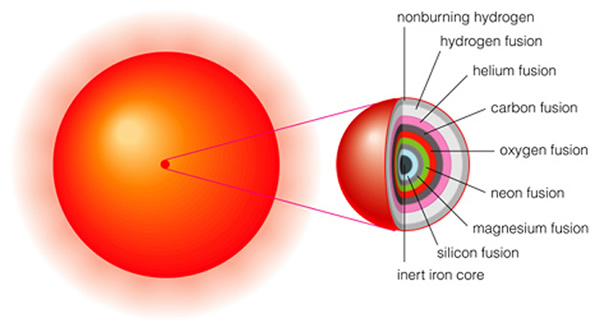
\includegraphics[scale=0.5]{figures/chapter1/high-mass-star-struct.jpeg}
        \caption{Illustration of the inner structure of a massive star before core-collapse. Credit: \href{http://astronomy.nmsu.edu/tharriso/ast110/}{Thomas Harrison | New Mexico State University.}}
        \label{fig:stellar_structure}
    \end{figure}
    Sooner than later, the iron core will collapse and trigger a supernova explosion, known as a ``\textit{core-collapse supernova}'', leaving behind a remnant in the form of a \textit{neutron star} or a \textit{black hole}.
    
    Lower-mass stars, on the other hand, have a different fate; since their cores never reach a high enough temperature to initiate carbon burning, they contract, developing a degenerate, inert core composed primarily of carbon and oxygen. The outer envelope, opposing the contraction of the inert core, expands, causing the star to cool as it enters the \textit{asymptotic giant branch} (AGB) H-R diagram.
    Simultaneously, strong stellar winds cause the outer layers to expel, forming a \textit{planetary nebula} and exposing the degenerate core. This naked core, known as a \textit{white dwarf}, is the final remnant left behind by such stars and no longer undergoes nuclear reactions but simply gradually cools down by radiating the residual heat.


    \subsubsection{Mixing in stellar interiors}
    The interior of a star is far from quiet. Equipped with a better understanding of how stars evolve, it is time to dive a little deeper into the more intricate dynamical processes that play a crucial role in their evolution. Here we will briefly present four fundamental mixing mechanisms caused by various instabilities.

    One of the most important mixing mechanisms that takes place in the stellar interior is that of \textit{convection}. It occurs when temperature variations across different layers induce density fluctuations, leading to buoyancy-driven fluid flows. This buoyancy-driven motion efficiently transports heavy elements through bulk motions, a phenomenon known as ``\textit{dredge-up}'', leading to the redistribution of material and energy. Essentially, a heated fluid parcel ascends due to buoyancy forces, while a colder parcel descends, taking its place. This convective process profoundly influences the star's structure, impacting phenomena like nucleosynthesis and magnetic field generation. Figure~\,\ref{fig:sun_granulation} depicts the granulation on our Sun's photosphere---a prominent illustration of the consequences of convection.
    
    \begin{figure}[ht!]
        \centering
        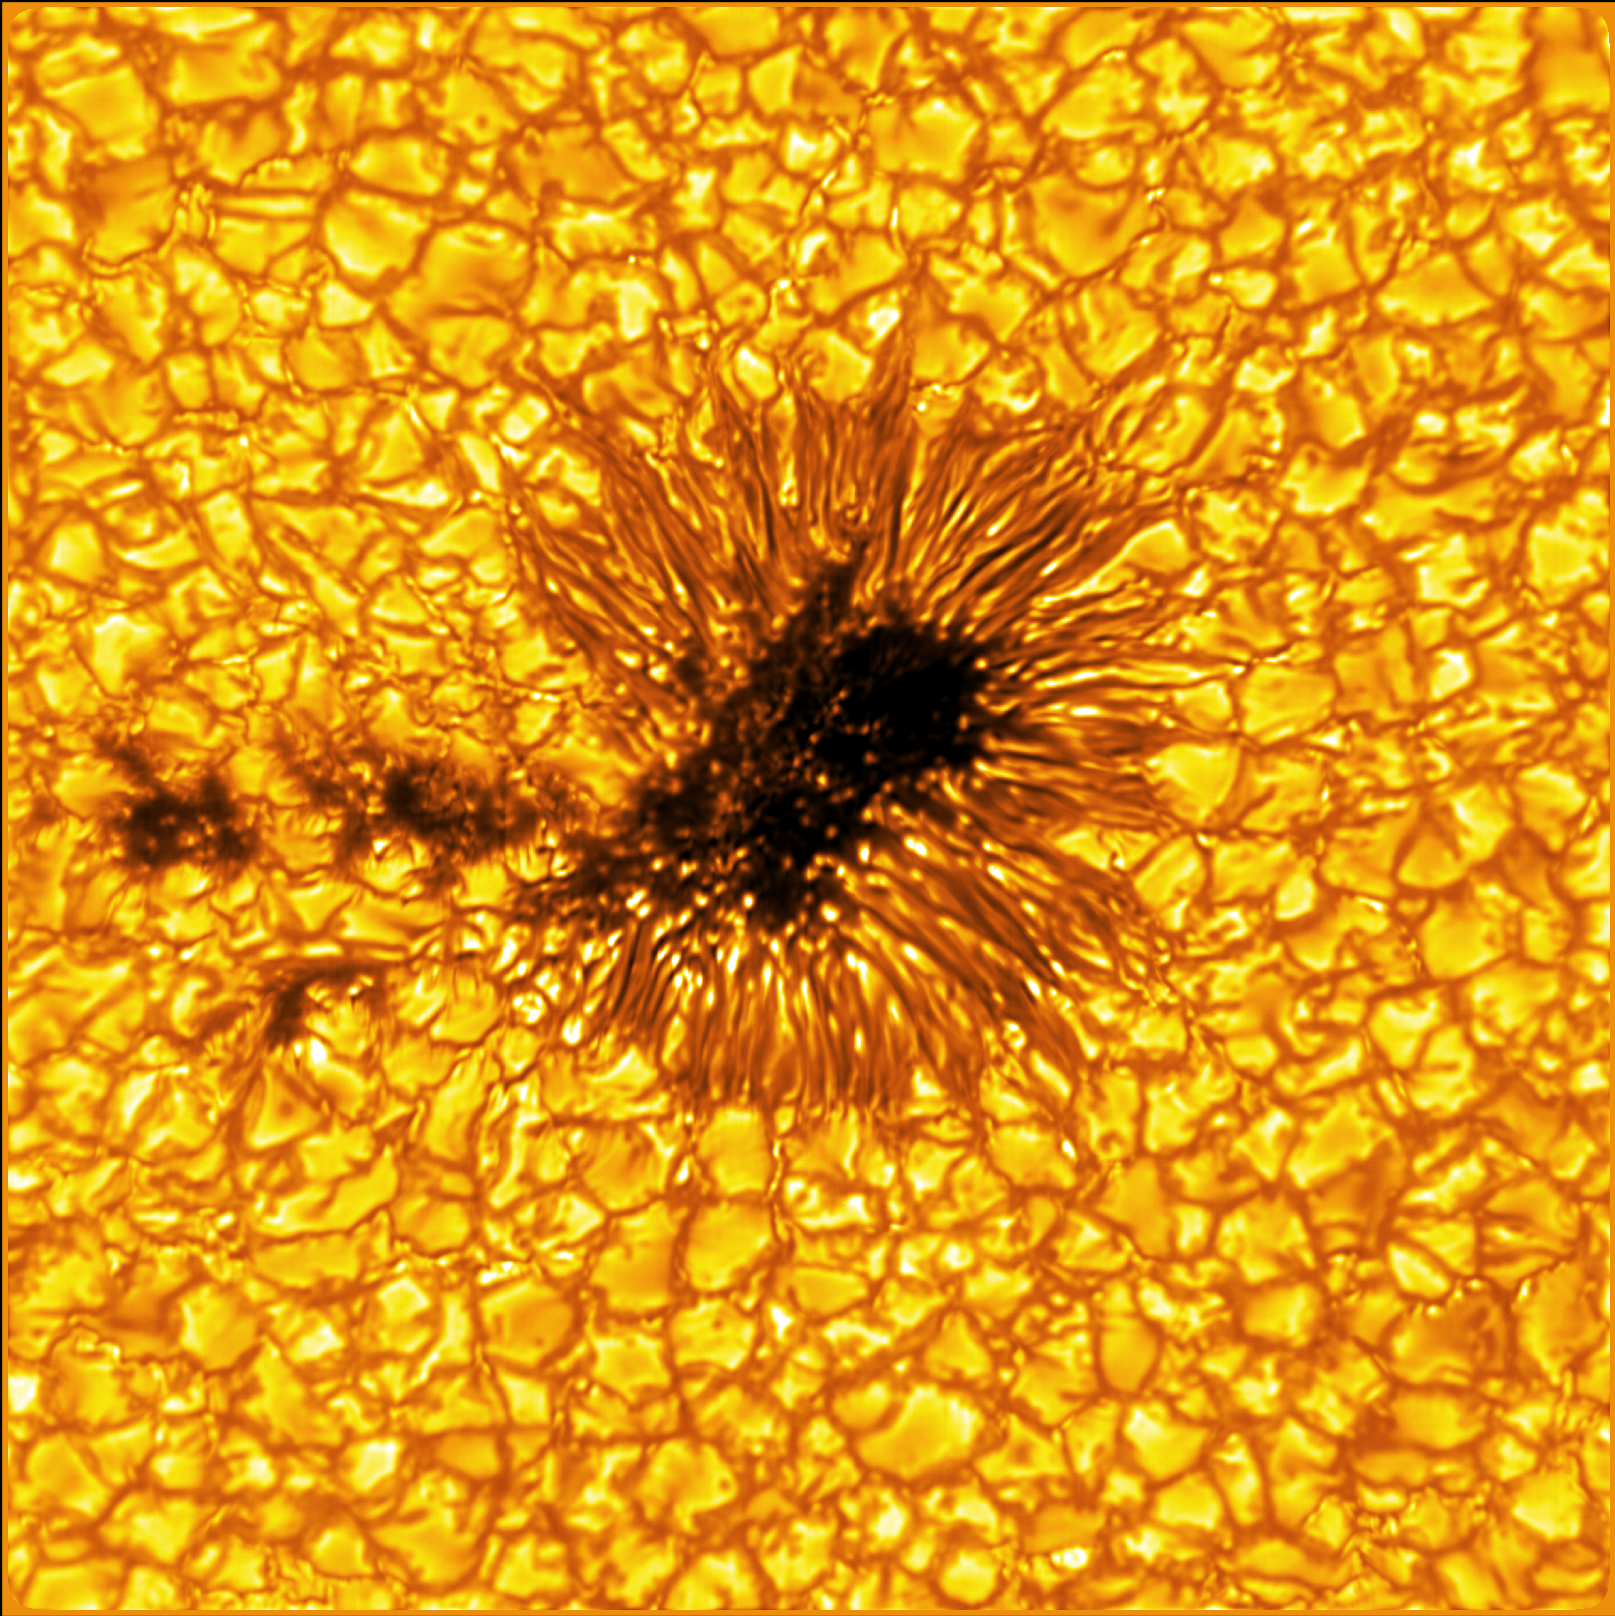
\includegraphics[scale=0.4]{figures/chapter1/sun_granulation.png}
        \caption{A captivating view of the Sun's photosphere revealing distinct granulations scattered across its surface. In the center, a large black sunspot stands out, its darkness attributed to a lower temperature caused by intense magnetic fields that disrupt the convective transfer of heat. This stark contrast highlights the dynamic interplay of convective processes and magnetic fields on the solar surface. Copyright: \href{https://nso.edu/}{National Solar Observatory}}
        \label{fig:sun_granulation}
    \end{figure}

    The stability of a layer against convection is determined by the \textit{Ledoux} criterion:
    \begin{equation}\label{eq:ledoux}
        \nabla_{\text{rad}} < \nabla_{\text{ad}} - \frac{\phi}{\delta} \nabla_{\mu}.
    \end{equation}
    In the case of chemically homogeneous layers ($\nabla_{\mu} = 0$), reduces to the \emph{Schwartzschild} criterion:	
    \begin{equation}\label{eq:schwarzschild}
        \nabla_{\text{rad}} < \nabla_{\text{ad}}.
    \end{equation}
    Here, $\nabla_\mathrm{rad}$ represents the radiative temperature gradient describing the logarithmic temperature variation with depth when energy is transported by radiation, $\nabla_\mathrm{ad}$ is the adiabatic temperature gradient defined similarly to $\nabla_\mathrm{rad}$ but for adiabatic compression or expansion, and $\nabla_\mu$ is the composition gradient accounting for variations in chemical composition within the medium.
    
    Modeling convection in astrophysical contexts is a notoriously difficult problem and poses significant challenges due to the complex, turbulent nature of convective flows. The inherent non-linearity and multi-scale behavior of convective processes make their accurate representation in numerical simulations demanding. One widely employed approach is the \textit{Mixing Length Theory} (MLT), which simplifies convective dynamics by introducing a characteristic length scale to describe the convective cells' average size and behavior. While MLT has been successful in certain applications, it has limitations in capturing the full complexity of convection, especially in regions with varying conditions. As a result, convection is often treated as a diffusive process in computational models, wherein the convective transport of energy, momentum, and chemical species is approximated using diffusion equations. This simplification facilitates numerical simulations but may overlook finer details of convective behavior, introducing a lot of uncertainties in our stellar evolution models.

    Another mixing process observed in stellar interiors is called \textit{semi-convection}, which is characterized by an intermediate state between full convection and radiative diffusion. This phenomenon occurs in regions where convective instability interacts with stratified layers, i.e. in regions that are stable to Ledoux criterion but unstable to Schwarzschild \citep[see][]{spruit:semiconvection}. Semi-convection contributes to the transport of both chemical elements and angular momentum, influencing the internal rotation profiles of stars and impacting their overall evolution.

    As we mentioned, the boundaries of a convective zone are determined by the Ledoux or Schwarzschild criteria. Nevertheless, \textit{convective overshooting} extends the impact of convective zones beyond their formal boundaries. As convective cells reach the boundaries of a convective region, they may overshoot and penetrate into adjacent stable layers due to their inertia until they lose all of their momentum. This overshooting process has implications for the extent of mixing in the stellar interior, affecting the transport of elements and altering the size of convective cores in evolving stars.
    
    Last but not least, in certain stellar environments, a phenomenon known as \textit{thermohaline} mixing manifests when there is a decrease in molecular weight with depth. This scenario often arises in binary systems undergoing accretion, creating stratified layers such as a helium layer overlying a hydrogen-rich one. As a consequence, the heavier elements tend to sink while the lighter materials ascend, leading to a restructuring of the mean molecular weight.

    

    \subsubsection{Effects of rotation}
    Thus far, we have silently operated under the assumption that the overview of stellar evolution provided relates solely to spherically symmetrical, non-rotating stars. However, rotation constitutes a crucial factor that profoundly impacts the evolution of stars and deserves to be discussed separately. 

    The inclusion of rotation introduces a (even more) dynamic aspect to stellar evolution, influencing various processes such as angular momentum transport, magnetic field generation, and the overall structure of a star. As stars form from rotating molecular clouds, the conservation of angular momentum plays a pivotal role in shaping their subsequent evolution. The rotation rate affects the size, shape, and internal distribution of matter within a star, influencing its overall stability and lifespan.

    Rotation induces various instabilities that significantly influence the mixing processes and internal dynamics of stars. The Eddington-Sweet circulation, for instance, arises due to the interaction between rotation and density gradients, leading to meridional flows that impact the transport of heat and various isotopes within the stellar interior. The dynamical shear instability and secular shear instability are additional rotational instabilities that can affect the internal shear profile of a star, influencing its overall stability and evolution. Additionally, the interplay between rotation and magnetic fields gives rise to phenomena like the solar dynamo, influencing the generation and modulation of the star's magnetic activity.

    Understanding the role of rotation-induced instabilities in stellar evolution is crucial for deciphering the observed diversity in stellar properties and behaviors. As stars age, their rotation rates can change due to processes like stellar winds and mass loss, further impacting their evolution. Therefore, a comprehensive exploration of stellar evolution necessitates a detailed examination of the influence of rotation and the associated instabilities.

    \subsubsection{Stellar winds}

    

    \subsection{Stellar Remnants}\label{sec:ch1:remnants}

    
    \subsubsection{White Dwarfs}


    \subsubsection{Neutron Stars \& Pulsars}


    \subsubsection{Black Holes}


    \subsection{Binary Evolution}\label{sec:ch1:binaries}

    \subsection{Explosive Stellar Transients}\label{sec:ch1:transients}


    \section{The Structure of Neutron Stars}\label{sec:ch1:ns_struct}

    \subsection{Equation of State}
    \subsection{Phase Transitions}
    \subsubsection{Construction of the Phase Transition}

    \section{Pulsar Astronomy}\label{sec:ch1:pulsar_astro}

    \subsection{Pulsar Timing}

    \section{Thesis Outline}
    



\end{document}